
%% manuscript produces a one-column, double-spaced document:
\documentclass[11pt,a4paper]{article}
%\documentclass[12pt, manuscript]%{aastex}
\usepackage{graphicx}
\usepackage{hyperref}

\usepackage{amsmath,amssymb,amsfonts}
\usepackage{subfig}
\usepackage{natbib, aas_macros}
\citestyle{aa}
\usepackage{setspace}
\usepackage{times}
\usepackage{rotating}
 \usepackage{fancyhdr}
\usepackage{booktabs}
\usepackage{gensymb}
\usepackage{lineno}
\usepackage{footnote}
\usepackage{tablefootnote}


%%% packages for pretty timeline %%%
%\usepackage[utf8]{inputenc}
%\usepackage[TS1,T1]{fontenc}
%\usepackage{fourier, heuristica}
\usepackage{array}
%\usepackage{graphicx}
\usepackage[x11names]{xcolor}
\usepackage{colortbl}
\usepackage{caption}
\usepackage{listings}
\usepackage{lmodern}
\usepackage[T1]{fontenc}
\newcommand{\foo}{\makebox[0pt]{\textbullet}\hskip-0.5pt\vrule width 1pt\hspace{\labelsep}}

%%%

%%%%%%%%%%%%%%%%text size and spacing%%%%%%
%%% Number equations according to section %%%
\numberwithin{equation}{section}

%%% text size %%%
\setlength{\topmargin}{10mm}
\addtolength{\topmargin}{-1in}
\setlength{\textheight}{262mm}
\setlength{\headsep}{5mm}
\setlength{\headheight}{0mm}
\setlength{\topskip}{0mm}
\setlength{\oddsidemargin}{-1in} %  set real left margin 0pt
\setlength{\evensidemargin}{-1in} % do
\addtolength{\oddsidemargin}{25mm} % odd page 25mm left margin
\addtolength{\evensidemargin}{15mm}% even page 15mm left margin
\setlength{\textwidth}{170mm}
%\setlength{\leftmargin}{-1 in}

\pagestyle{fancy}
\lhead[\it\scriptsize \leftmark]{}
\chead[]{}
\rhead[]{\it \scriptsize \rightmark}
\renewcommand{\headrulewidth}{0.4pt}
\renewcommand{\footrulewidth}{0pt}
\renewcommand{\baselinestretch}{1.}
\renewcommand{\bibname}{References}

\doublespacing

\title{Doctoral Thesis Abstract\\
AKARI and Spinning Dust Emission\\
}

\author{Aaron Christopher Bell}

\begin{document}
\maketitle
\singlespacing

The anomalous microwave emission (AME) still lacks a conclusive explanation.  This excess of emission, roughly between 10 and 50~GHz, tends to defy attempts to explain it as synchrotron or free-free emission. The overlap with frequencies important for cosmic microwae background explorations, combined with a strong correlation with interstellar dust, drive cross-disciplinary collaboration between interstellar medium and obervational cosmology. The apparent relationship with dust has prompted a ``spinning dust'' hypothesis:  electric dipole emission by rapidly rotating, small dust grains. Magnetic dipole emission by grains with magnetic inclusions (``magnetic dust''), while less suppported, has not been ruled out. Even assuming a spinning dust scenario, we are far from concluding which category of dust contributes. The typical peak frequency range of the AME profile implicates grains on the order of ~1nm. This points to polycyclic aromatic hydrocarbon molecules (PAHs). We use data from the AKARI/Infrared Camera (IRC)\cite{irc07,ishihara10}, due to its thorough PAH-band coverage, to compare AME from the Planck Collaboration \cite{planck15X}. astrophysical component separation product) with infrared dust emission. We look also at infrared dust emission from other mid IR and far-IR bands (see Fig.~\ref{fig:Filter_coverage_example_full})
  \begin{figure}
    \centering
    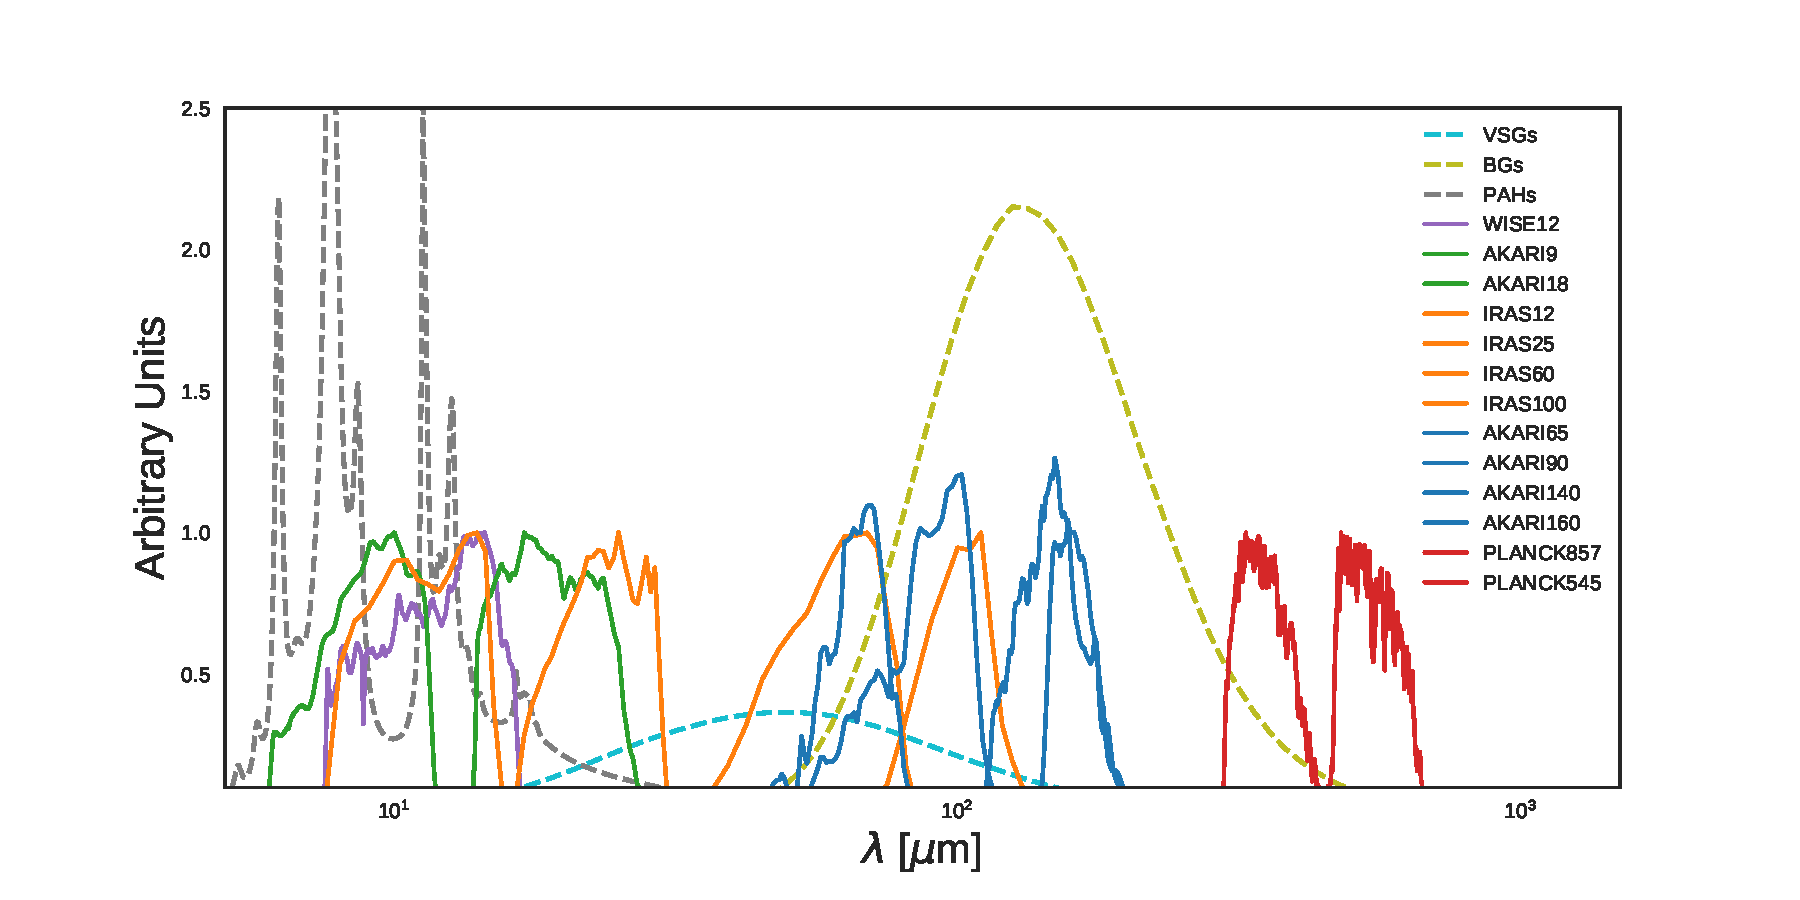
\includegraphics[width=\textwidth]{../Plots/ch_datasources/Filter_coverage_example_full.pdf}
    \caption{Relative spectral response curves of the bands used in this study. Expected dust emission components, assuming the dust SED model by \citep{dustem11} are also shown. The components are summarized as emission from big grains (BGs, dashed yellow line), emission from very small grains (VSGs, dashed blue line), and emission from PAHs (dashed grey line).}
    \label{fig:Filter_coverage_example_full}
  \end{figure}
 The results and discussion contained here apply to an angular scale of approximately 1$^{\circ}$. In general, our results support an AME-from-dust hypothesis. We look both at $\lambda$~Orionis, a region highlighted for strong AME, and find that certainly dust mass correlates with AME, and that PAH-related emission in the AKARI/IRC 9~$\mu$m band may correlate slightly more strongly (see Fig.~\ref{fig:bootstrap_vs_AME}).
   \begin{figure}
     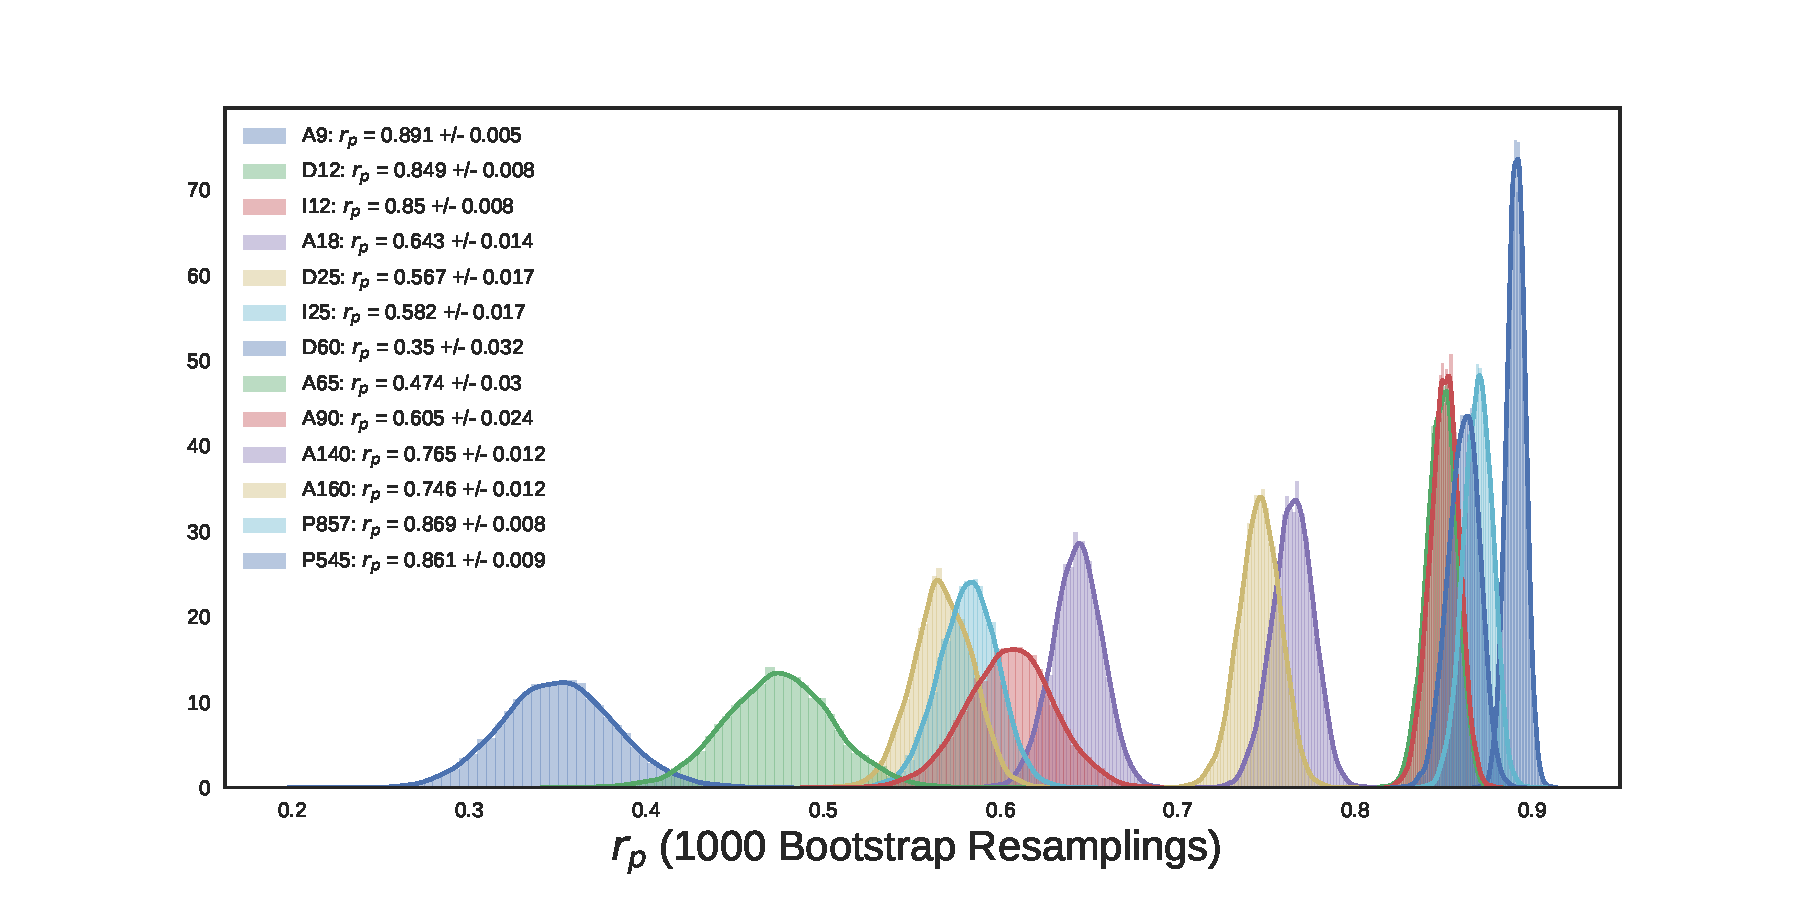
\includegraphics[width=\textwidth,trim={3cm 0.25cm 2.5cm 1cm},clip]{../Plots/ch_lori/bootstrap_vs_AME_pearson_i10000.pdf}
     \centering
     \caption{Re-sampled (Bootstrap) Pearson correlation ($r_{p}$) tests for IR emission in $\lambda$~Orionis vs. AME. Each band's $r_p$ distribution is shown in a different color (the same color scheme for both plots). Bootstrapping is an iterative resampling and retesting of the data, mitigating the effects of noise and outliers. The width of each distribution esimates the error in $r_{p}$. The legend gives the mean and standard deviation of $r_{p}$. 'A' indicates AKARI; 'D', DIRBE; 'I', IRAS, and 'P' Planck. The number after each letter indicates the band central nominal wavelength in microns (or frequency in GHz, in the case of the Planck bands.)}
     \label{fig:bootstrap_vs_AME}
   \end{figure}
 These results are compared to an all-sky analysis, where we find that potential microwave emission component separation imperfections among other issues, make an all-sky, delocalized comparsion very challenging. In any case the AME-to-dust correlation persists even in the all-sky case, but tests of relative variations from different dust SED components are largely inconclusive. We emphasize that future efforts to understand AME should focus on individual regions, and a detailed comparsion of the PAH features with the variation of the AME SED. Further all-sky analyses seem unlikely to help resolve this issue. Non-PAH carriers of the AME, such as nanosilicates, cannot be ruled out either.

\small
\bibliographystyle{apj}
\bibliography{reference}
\end{document}
